\documentclass[border=10pt]{standalone}
\usepackage{tikz}
\usetikzlibrary{arrows.meta, positioning, calc, fit, backgrounds}

\begin{document}

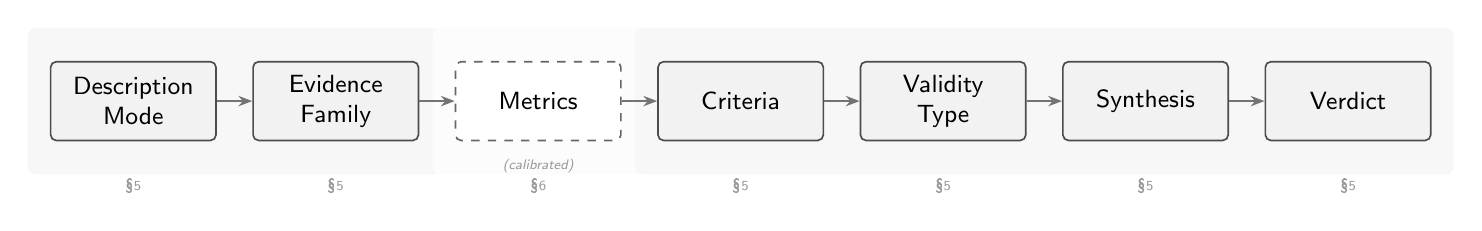
\begin{tikzpicture}[
    fbox/.style={
        rectangle, rounded corners=2pt,
        draw=black!70, fill=black!5,
        minimum height=1.0cm, minimum width=2.1cm,
        font=\sffamily\small, align=center,
        line width=0.6pt,
    },
    mbox/.style={
        rectangle, rounded corners=2pt,
        draw=black!60, fill=white,
        minimum height=1.0cm, minimum width=2.1cm,
        font=\sffamily\small, align=center,
        line width=0.6pt, dashed,
    },
    arr/.style={-{Stealth[length=5pt]}, line width=0.7pt, black!55},
    seclabel/.style={font=\sffamily\tiny\color{black!40}},
]

% === PIPELINE: single row ===
\node[fbox] (mode) at (0, 0) {Description\\Mode};
\node[fbox, right=0.45cm of mode] (family) {Evidence\\Family};
\node[mbox, right=0.45cm of family] (metrics) {Metrics};
\node[fbox, right=0.45cm of metrics] (criteria) {Criteria};
\node[fbox, right=0.45cm of criteria] (type) {Validity\\Type};
\node[fbox, right=0.45cm of type] (synthesis) {Synthesis};
\node[fbox, right=0.45cm of synthesis] (verdict) {Verdict};

% Arrows
\draw[arr] (mode) -- (family);
\draw[arr] (family) -- (metrics);
\draw[arr] (metrics) -- (criteria);
\draw[arr] (criteria) -- (type);
\draw[arr] (type) -- (synthesis);
\draw[arr] (synthesis) -- (verdict);

% Section labels underneath
\node[seclabel, below=10pt of mode] {\textsection 5};
\node[seclabel, below=10pt of family] {\textsection 5};
\node[seclabel, below=10pt of metrics] {\textsection 6};
\node[seclabel, below=10pt of criteria] {\textsection 5};
\node[seclabel, below=10pt of type] {\textsection 5};
\node[seclabel, below=10pt of synthesis] {\textsection 5};
\node[seclabel, below=10pt of verdict] {\textsection 5};

% Calibrations note
\node[font=\sffamily\tiny\itshape\color{black!40}, below=3pt of metrics] {(calibrated)};

% Background regions
\begin{scope}[on background layer]
    % §5 left
    \node[fit=(mode)(family), inner sep=8pt, inner ysep=12pt, fill=black!3, rounded corners=3pt] {};
    % §6
    \node[fit=(metrics), inner sep=8pt, inner ysep=12pt, fill=black!1, rounded corners=3pt] {};
    % §5 right
    \node[fit=(criteria)(verdict), inner sep=8pt, inner ysep=12pt, fill=black!3, rounded corners=3pt] {};
\end{scope}

\end{tikzpicture}

\end{document}
